\section{Background}

This syntax and explanation is a combination of ideas from from many sources \cite{Lyu2021,Li2020,Mei2006,Yu2005,Kruger2018}.

\subsection{Macroscopic Fluid Dynamics}

Traditionally, fluid dynamics problems are 
modelled by numerically solving some 
differential equations over the fluid's domain.
Fluid dynamics conserve mass, so solvers should account for the law of conservation of mass
\begin{align}
  \frac{\partial \rho}{\partial t} + \nabla \cdot (\rho \bm{u}) &= 0
\end{align}
where $\rho$ is density and $\bm{u}$ is velocity. 
Essentially, the change in density at any point should be 
balanced by mass entering or leaving that region.
Another common equation to account for is the Navier-Stokes momentum equation
\begin{align}
\frac{\partial}{\partial t} (\rho \bm{u}) 
+ \nabla \cdot (\rho \bm{u} \times \bm{u}) &= 
- \nabla \bm{p} + \nabla \cdot \sigma + F
\end{align}
where $\bm{p}$ is pressure, $\sigma$ is shear stress tensor, and $F$
represents any external forces like gravity. 
This is another conservation law that relates several \textit{macroscopic}
quantities of fluid.
Fluids dynamics are the emergent behavior of the \textit{microscopic} 
behavior of molecules.
Macroscopic quantities, like pressure, are an observed average of 
microscopic quantities.
Even fluid velocity, in the sense we're interested in, 
is a macroscopic quantity.

Many other approaches to modelling fluid dynamics,
like finite volume, finite element, and even 
smoothed particle hydrodynamics(?)
seek to solve for macroscopic 
fields like $\bm{u}$ and $\bm{p}$.

\subsection{LBM}
The lattice Boltzmann method (LBM) is a collection of techniques for
numerically modelling fluid dynamics that solves for microscopic quantities.
In particular, LBM solves the numerically solves 
the lattice Boltzmann equation
\begin{align}\label{eqn:cont_lbm}
  \frac{\partial f}{\partial t} + \bm{v} \cdot \nabla f = \Omega(f) + F\nabla_{\bm{v}} f
\end{align}
LBM solves this equation for a probability distribution $f(x, \bm{v}, t)$ which
describes the probability of a particle to be at point $x$, traveling with macroscopic velocity $\bm{v}$ at time $t$.

The discretization used in LBM to numerically solve \ref{eqn:cont_lbm} 
has two components.
First the fluid domain, space, is 
discretized onto a
grid of points $x \in \delta_x \mathbb{Z}^D$
where $\delta_x$ is the spacing between points in world coordinates
and $D$ is the spatial dimension ($3$ for most of our examples.)

The second part is discretizing the possible velocities a particle 
could be traveling in. 
Each point has a finite number, $Q$, of directions it can travel in, $c_i$.
These directions relate points in the grid and form the titular lattice.
These lattices are typically denoted by $D\#Q\#$.
Common lattices include $D2Q9$ (a) or $D3Q27$ (b), see below (figure from \cite{Li2020}.)
\begin{center}
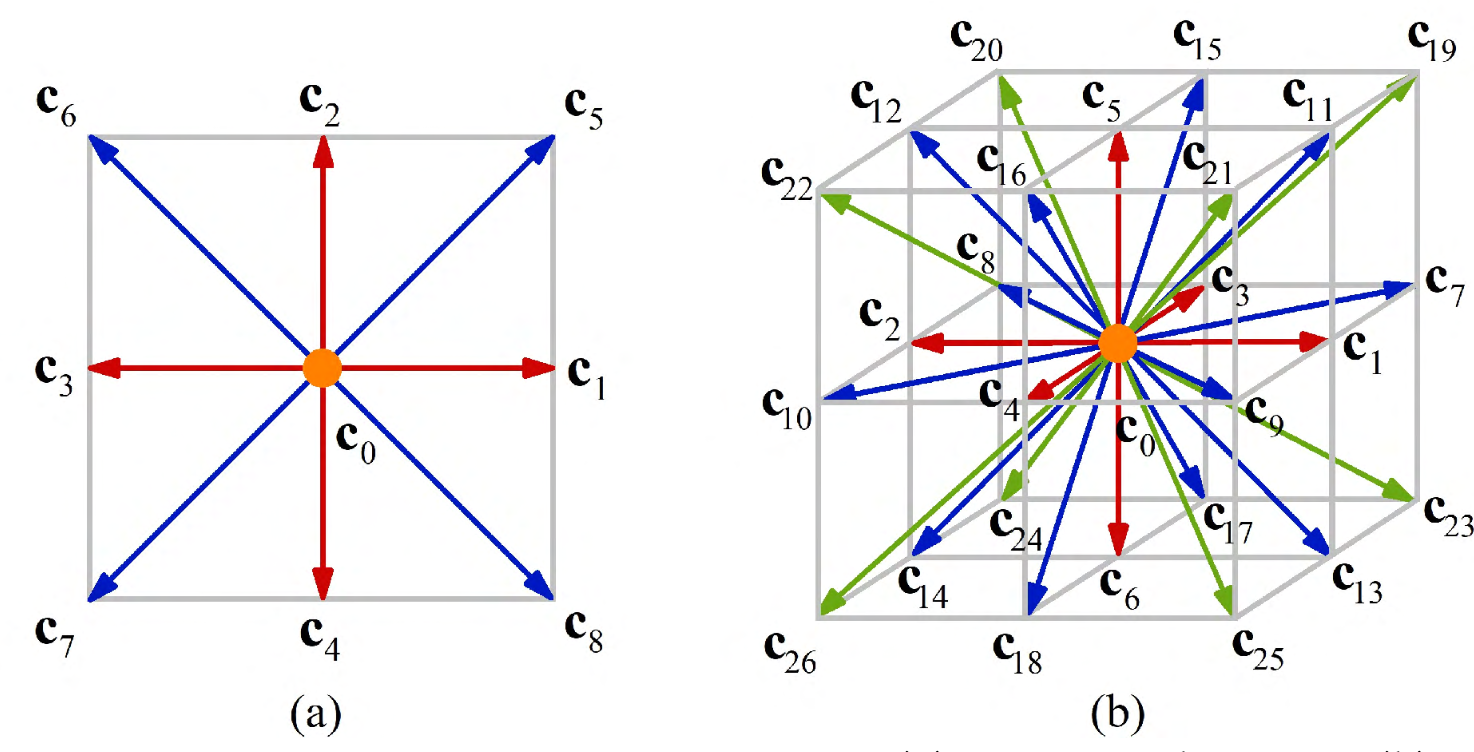
\includegraphics[width=0.6\linewidth]{lattice_figure.png}
\end{center}

There are several subtleties with this discretized velocity space, 
$\mathbb{V} \equiv \mathbb{R}^Q$. 
\begin{outline}
\1 We refer to the each microscopic velocity component with 
$f_i(x, t)$ for $i \in 0..Q - 1$.
\1 Each of these $f_i(x, t)$ values is a probability that there is a particle traveling with at a fixed velocity, $c_s$, in the direction $c_i$.
\1 Integrals over microscopic velocities can recover macroscopic properties.
In this context we refer to these integral properties as moments, 
and they are calculated as sums. 
For example, pressure and momentum (?) are the zeroth and first moment 
of the microscropic velocity distribution.
\begin{align}
  \rho(x, t) &= \sum_{i = 0}^{Q - 1} f_i(x, t) \\
  \rho(x,t)u(x,t) &= \sum_{i = 0}^{Q - 1}c_i f_i(x, t)
\end{align}
\end{outline}

 


\subsection{LBM Implementations}

There were several lattice boltzman implementations that were helpful to me.
\begin{outline}
  \1 A literate implementation of LBM using SymPy and CUDA \cite{web:literate_lbm}
  \1 An interactive 2D implementation written in Rust and WGPU \cite{web:lbm-web}.
  \2 While this was an important resource in that it demonstrated 
  the feasibility of what I wanted to do, 
  my implementation shares no code or even structural similarities 
  with this implementation.
  \1 A CPU only LBM implementation written in Rust \cite{web:lbm-rs}.
  \2 The interface and workflow of this tool was exactly what I wanted, but it didn't use the GPU at all.
  \1 An implementation of MRT LBM from \cite{Yang2022} is available on \href{https://github.com/yjhp1016/taichi_LBM3D/}{github}.
\end{outline}

WGPU on my M1 Max GPU has a max storage buffer size of $4.29$ gb.
That is sufficient to hold a billion floating point numbers.
Normally, the distributions are stored in one large contiguous allocation 
as a $D+Q$ dimensional array.
In such setup, this would limit us around $350^3$ lattice points.

By storing each direction in a separate buffer, we incur some additional expense but raise our maximum problem size to $115.83$ gb.

I opted to take on additiona

\subsection{MRT}

\subsection{CMT}

This is adapted from equation 35 from the supplemental materials of \cite{Li2020}, and equation 9 from \cite{De2017} 
\begin{align*}
m_{0} &= \{  1 \},\\
m_{1} &= \{  \bar{c}_{j,x} \},
m_{2} = \{  \bar{c}_{j,y} \},
m_{3} = \{  \bar{c}_{j,z} \},\\
m_{4} &= \{  \bar{c}_{j,x} \bar{c}_{j,y} \},
m_{5} = \{  \bar{c}_{j,x} \bar{c}_{j,z} \},
m_{6} = \{  \bar{c}_{j,y} \bar{c}_{j,z} \},\\
m_{7} &= \{  \bar{c}_{j,x}^2 - \bar{c}_{j,y}^2 \},
m_{8} = \{  \bar{c}_{j,x}^2 - \bar{c}_{j,z}^2 \}, \\
m_{9} &= \{  \bar{c}_{j,x}^2 + \bar{c}_{j,y}^2 + \bar{c}_{j,z}^2 \},\\
m_{10} &= \{ \bar{c}_{j,x} \bar{c}_{j,y}^2 + \bar{c}_{j,x} \bar{c}_{j,z}^2 \},
m_{11} = \{ \bar{c}_{j,x}^2 \bar{c}_{j,y} + \bar{c}_{j,y} \bar{c}_{j,z}^2 \},\\
m_{12} &= \{ \bar{c}_{j,x}^2 \bar{c}_{j,z} + \bar{c}_{j,y}^2 \bar{c}_{j,z} \},
m_{13} = \{ \bar{c}_{j,x} \bar{c}_{j,y}^2 - \bar{c}_{j,x} \bar{c}_{j,z}^2 \},\\
m_{14} &= \{ \bar{c}_{j,x}^2 \bar{c}_{j,y} - \bar{c}_{j,y} \bar{c}_{j,z}^2 \},
m_{15} = \{ \bar{c}_{j,x}^2 \bar{c}_{j,z} - \bar{c}_{j,y}^2 \bar{c}_{j,z} \},\\
m_{16} &= \{ \bar{c}_{j,x} \bar{c}_{j,y} \bar{c}_{j,z} \},\\
m_{17} &= \{ \bar{c}_{j,x}^2 \bar{c}_{j,y}^2 + \bar{c}_{j,x}^2 \bar{c}_{j,z}^2 + \bar{c}_{j,y}^2 \bar{c}_{j,z}^2 \},\\
m_{18} &= \{ \bar{c}_{j,x}^2 \bar{c}_{j,y}^2 + \bar{c}_{j,x}^2 \bar{c}_{j,z}^2 - \bar{c}_{j,y}^2 \bar{c}_{j,z}^2 \}, \\
m_{19} &= \{ \bar{c}_{j,x}^2 \bar{c}_{j,y}^2 - \bar{c}_{j,x}^2 \bar{c}_{j,z}^2 \},\\
m_{20} &= \{ \bar{c}_{j,x}^2 \bar{c}_{j,y} \bar{c}_{j,z} \},
m_{21} = \{ \bar{c}_{j,x} \bar{c}_{j,y}^2 \bar{c}_{j,z} \},\\
m_{22} &= \{ \bar{c}_{j,x} \bar{c}_{j,y} \bar{c}_{j,z}^2 \},\\
m_{23} &= \{ \bar{c}_{j,x} \bar{c}_{j,y}^2 \bar{c}_{j,z}^2 \},
m_{24} = \{ \bar{c}_{j,x}^2 \bar{c}_{j,y} \bar{c}_{j,z}^2 \},\\
m_{25} &= \{ \bar{c}_{j,x}^2 \bar{c}_{j,y}^2 \bar{c}_{j,z} \},\\
m_{26} &= \{ \bar{c}_{j,x}^2 \bar{c}_{j,y}^2 \bar{c}_{j,z}^2 \},\\
\end{align*}

The first $9$ moments have physical interpretations,
and their relaxation rates follow \cite{Li2020, De2017}.
\begin{align}
  r_0 &= 0, \nonumber \\
  r_i &= 2, \text{ for } i = 1,2,3 \nonumber \\
  r_i &= (3v + 1 / 2)^{-1}, \text{ for } i = 4,\ldots, 9 \label{eqn:kv_rate}
\end{align}
Setting the relaxation rates for higher order moments 
is an area of active research.
In \cite{Li2020} an adaptive scheme for setting these rates
per $x$ per timestep was described.
I didn't attempt to implement that, instead I fixed them as contants

was related to this 
issue.
In \cite{Li2018} the following viscosities were proposed for
these higher order relaxation rates to use with equation \ref{eqn:kv_rate}
\begin{align*}
  v_i &= 0.005, \text{ for } i = 9,\ldots, 16 \\
  v_i &= 0.007, \text{ for } i = 17, \ldots, 22 \\
  v_i &= 0.009, \text{ for } i = 26 
\end{align*}


\cite{Suga2015} has $D3Q27$ MRT explicitly written out!

\cite{Hennig2023} presents lbmpy for generating MRT collision operators.

\cite{Li2018} shows how to do spatial adaptivity I think.
